\subsection{ESP32 TTGO T-Display}

The TTGO T-Display ESP32 Development Board is a compact development board based on the ESP32 Microcontroller, which is widely used for embedded systems and Internet of Things (IoT) applications. The board integrates Wi-Fi and Bluetooth connectivity, allowing devices to communicate wirelessly with other systems or the internet. In addition to the microcontroller, the board includes a small built-in color display, making it convenient for projects that require real-time visual output without needing an external screen.

\begin{figure}[ht]
    \centering
    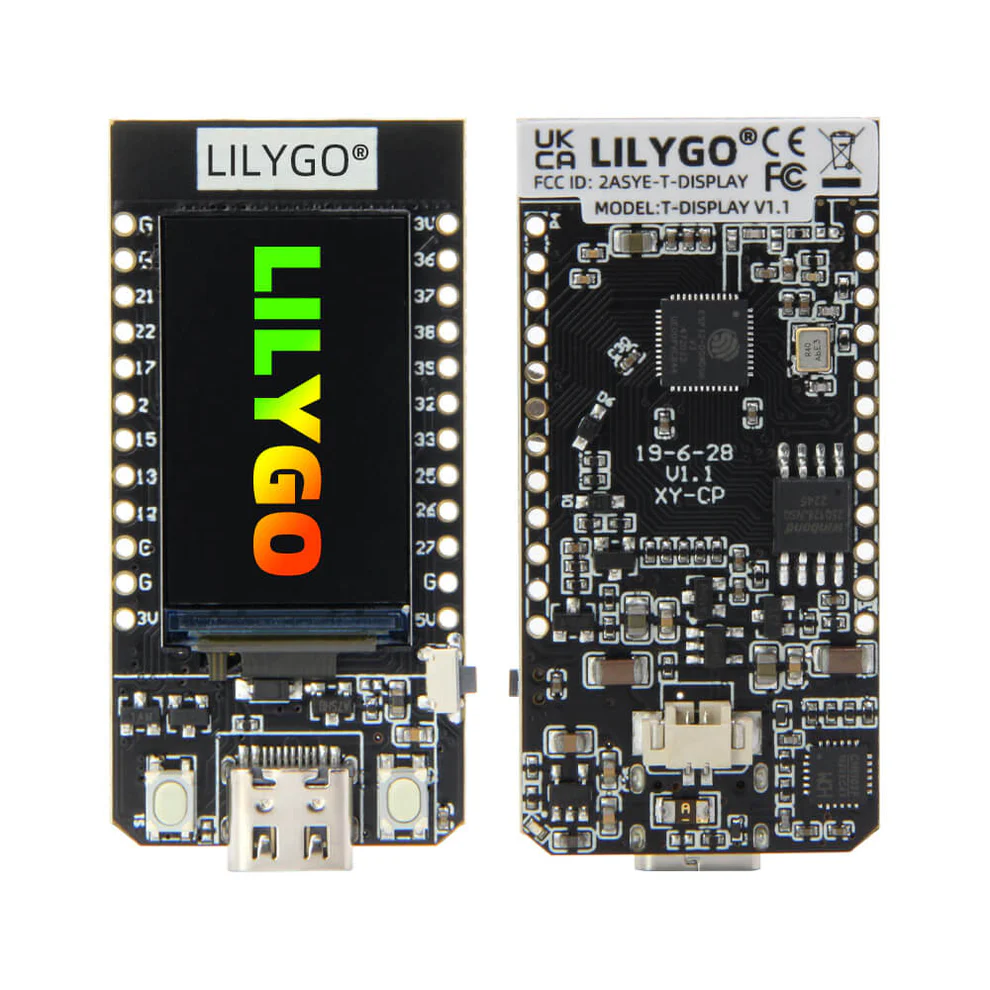
\includegraphics[width=0.4\textwidth]{components/image/esp32ttgo_product.png}
    \caption{ESP32 TTGO T-Display development board \cite{esp32ttgo_product}.}
    \label{fig:esp32ttgo_product}
\end{figure}

The board also provides GPIO pins for connecting sensors, actuators, and other electronic components. With its micro-USB interface for programming and power, the board is easy to set up and can be programmed using development environments such as Arduino IDE or PlatformIO.

As for power supply, the TTGO T-Display can be powered via several methods \cite{esp32ttgo_product}, including:

\begin{itemize}
    \item USB-C with 5V input
    \item LiPo battery providing 3.7V input
    \item External 5V supply through the VIN pin
\end{itemize}

\begin{figure}[ht]
    \centering
    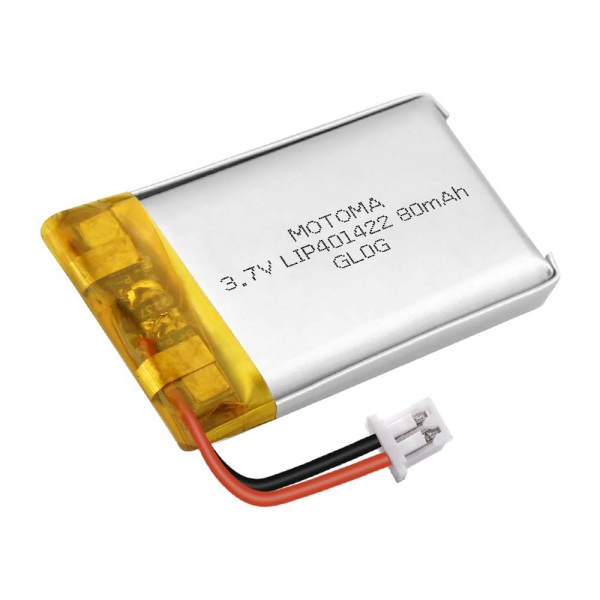
\includegraphics[width=0.3\textwidth]{components/image/lipo3.7v_product.png}
    \caption{3.7V LiPo battery for ESP32 TTGO T-Display \cite{lipo_motoma}.}
    \label{fig:lipo3.7v_product}
\end{figure}

Within the scope of this project, the LiPo battery power supply method was chosen for its portability and convenience, allowing the device to operate independently without being tethered to a power source. Together with the circuit itself, the battery is housed within a custom 3D-printed enclosure, allowing for a cohesive and functional design that meets the requirements of the project.